\documentclass[english,11pt]{article}
\usepackage[T1]{fontenc}
\usepackage[utf8]{inputenc}
\usepackage{graphicx}
\usepackage{geometry}
\usepackage{caption}
\usepackage{subcaption}
\usepackage{babel}
\usepackage{amsmath}
\usepackage[nottoc,numbib]{tocbibind}
\usepackage{verbatim}
\usepackage{hyperref}
\numberwithin{equation}{section}

\begin{document}

\title{Wireless Sensor 4 Assessed Exercise}
\author{Motiejus Jakštys}
\date{13 March 2012}

\maketitle
\pagebreak
\tableofcontents
\pagebreak

\section{Introduction}

\subsection{Identification}

This document is the report of the Wireless Sensor Networks 4 Assessed Exercise.
It consits of the following:

\begin{enumerate}
    \item TinyBlog application in TinyOS.
    \item BaseStation application in TinyOS.
    \item Client application in Python.
\end{enumerate}

\section{System design}

For TinyBlog the following applications were used:
\begin{itemize}
    \item ActiveMessageC, RadioControl and AMReceiverC for receiving radio
        packets.
    \item AMSenderC for sending radio packets.
    \item LedsC for notifications about system status (blinking leds).
    \item TimerMilliC for internal queue management.
    \item SensirionSht11C for sensing environment temperature.
\end{itemize}

For wiring diagram please refer to figure~\ref{fig:wiring_diagram}.

\begin{figure}
    \centering
    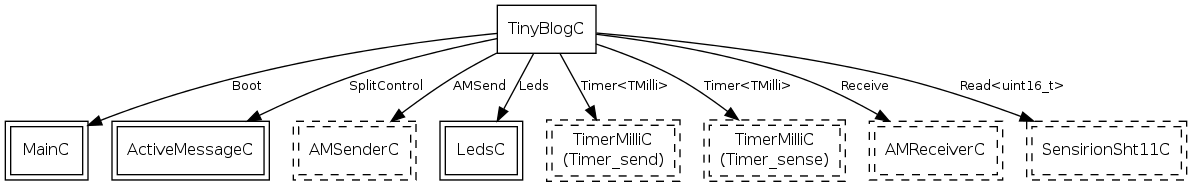
\includegraphics[width=\textwidth]{TinyBlogAppC.png}
    \caption{TinyBlogAppC wiring diagram}
    \label{fig:wiring_diagram}
\end{figure}

\section{Test methodology}

While the system looks fairly simple, it has a lot of moving parts, which have
to be tested well separately and together.

First of all, having modular components is a crucial must-have in order to be
able to properly test them. For that reason as much code as possible must be
abstracted from TinyOS and NesC, so it can be tested using standard C testing
components.

Once components are solid (well tested separately), it is time to test how well
they behave together. This means running the whole application and executing a
few sample scenarios.

Generally, testing will be done in three ways:
\begin{enumerate}
    \item Using standard C testing techniques on a desktop machine (or continous
        integration server).
    \item Using fully automated simulator (TOSSIM)
    \item Manual tests
\end{enumerate}

In the further chapters I will go into more detail how they should be done for
TinyBlog application.

\subsection{Component testing}

First all components should be tested separately using classic unit tests. Like
mentioned before, unit tests should not require any TinyOS environment.

Here are a few examples how certain parts of TinyBlog can be tested in unit
tests.

\subsubsection{Circular buffer tests}

Circular buffer tests should cover a few scenarios: test adding items,
overflowing the buffer and trying to send more messages that the buffer has.
Document and test its API. Logic of the module is fairly simple and without many
corner cases, so unit tests will be sufficiently extensive and this module will
not require more attention besides having up-to-date unit tests.

\subsubsection{Directed-diffusion routing}

Routing is much more complicated than circular buffer, therefore more extensive
test approach is needed.

Routing should be encapsulated in a library which does depend on neither NesC
nor TinyOS. All "send message" calls should be abstracted in a way that routing
library should be in plain C, therefore executable on a commodity machine.
"Send message", "receive message" calls should be easy to mock. In other words,
the library must give tools to insert user's implementation of the mentioned
commands.

Once the routing libray is written in NesC-and-TinyOS-independent way, it is
possible to extensively test it. There should be two kind of tests. First, a
series of standard unit tests, which model a few scenarios and verify that the
system works as expected. These tests are thought by human and normally cover
most of the cases.

In reality many component tests go as far as human-writen unit tests. However,
human testing suffers from one limitation: humans are lazy. Complex systems
explode in states, and writing very many different transitions of a complex
state machine is not feasible for a human. To tackle this problem another
approach was developed: model-based testing of stateful
systems\cite{model-testing}. Briefly saying, the test harness gives a model of
the system that is about to be tested, and the property-based testing tool
generates these state transitions at the same time verifying that the model
behaves correctly.

While this might sound initially complicated, but it is not. Testing routing is
a very good use case for property-based model testing. Here I will briefly
describe an example model for testing diffusion based routing.

\begin{description}
    \item[Initial state:] zero nodes.
    \item[Possible state transitions:]
        \begin{enumerate}
            \item Add node.
            \item Remove random node.
            \item Change noise/throughput of a link.
            \item Send message between two random nodes.
        \end{enumerate}
    \item[Postconditions] is the mechanism for ensuring the model behaves how it
        is intended. For example, if the message was sent from X to Y, it must
        eventually arrive to Y (given that there is a path between them).
\end{description}

Given that model to the tool, it will interact with it in many random ways and
will create the huge number of states which we were aiming for.

\subsubsection{Tweeter tests}

While initial Tweeter requirements are very basic, it is likely that they will
become more sophisticated while the program (cluster) matures. So it is
important to write tests for tweeting/following/etc logic from day 0.

Tweeter can also be modelled as a state machine, and can be tested using
property-based model testing techniques.

\subsection{Integration tests}

The goal is to execute the tests as frequently as possible in the development
cycle. This is easiest done in a simulator: once the simulation script is
written, it is quite easy to verify the correct behaviour of the system. What is
more, since the test is executed by a computer, the test case can be very long
and complicated.

An example test scenario. Add 100 motes to a network, make a few of them follow
each other (ideally in different corners of the network, so routing is not
trivial), and start tweeting. In the end number of hops should be calculated and
verified, as well as the "business" behaviour of following, tweeting and
retweeting.

\subsection{Acceptance tests}

When the product is ready for shipping, an extensive acceptance test suite must
be executed. Usually acceptance tests are superset of integration tests, but
with actions that must be executed by humans (i.e. manually). Since it is common
to all software-engineering projects and has nothing specific to TinyBlog
application, I will not go to this part in detail.

\subsection{Host-Mote communication}

Communication between host and mote is done as follows:
\begin{enumerate}
    \item \texttt{tinyblog.py} connects to serial forwarder.
    \item serial forwarder connects to serial port and talks to BaseStation
        (included in the archive)
    \item BaseStation forwards messages received from \texttt{tinyblog.py} to
        the user's mote.
\end{enumerate}

\begin{thebibliography}{9}

    \bibitem{model-testing}

        Broy, M.; Jonsson, B.; Katoen, J.-P.; Leucker, M.; Pretschner, A.
        (Eds.). \emph{Model-Based Testing of Reactive Systems}, ISBN
        978-3-540-26278-7

\end{thebibliography}
\end{document}
